\subsection{Datamodel}
Een van de belangrijkste doelen van de afstudeeropdracht is om een nieuw datamodel te maken voor een CMS-systeem.
Dit datamodel moet veel verschillende soorten datastructuren kunnen ondersteunen en deze kunnen presenteren op een klant zijn website.
Het huidige CMS van Snakeware doet dit door middel van een complexe structuur.
Deze structuur zorgt ervoor dat het moeilijk is om nieuwe functionaliteit toe te voegen en dat het systeem lastig is te onderhouden.

\whitespace
Daarom heeft het nieuwe datamodel twee belangrijke uitgangspunten om de pijnpunten van het oude CMS te voorkomen.
Het datamodel moet generiek blijven, zodat er veel verschillende datastructuren in opgeslagen kunnen worden.
Door het datamodel generiek en flexibel te houden hoeft het systeem niet uitgebreid te worden om een nieuwe datastructuren te ondersteunen.
Verder moet de structuur van het datamodel simpel blijven zodat het makkelijk te onderhouden is.
Om deze doelen te bereiken is er gebruik gemaakt van de volgende concepten.

\whitespace
\textbf{Fields}

\whitespace
Content op websites bestaan uit kleinere stukken data/ content.
Fields representeren de kleinste laag content op een website. 
Hierbij kun je denken aan een stukje tekst of aan een nummer op een site.
Om bij fields een beter beeld te schetsen is er een stuk van de Snakeware website gebruikt als voorbeeld.
In figuur \ref{fig:VisualisationFields} is te zien  waar fields zich plaats vinden in de content.

\whitespace[2]
\begin{graphic}
    \captionsetup{type=figure}
    \caption{Visualisatie van fields}
    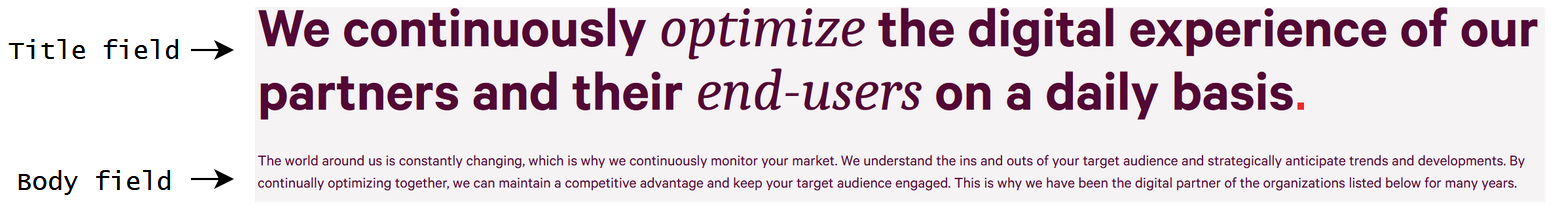
\includegraphics[scale=0.35]{VisualisationFields.png}
    \label{fig:VisualisationFields}
\end{graphic}

\whitespace
\textbf{Items}

\whitespace
Om een samenhangend stuk content op te stellen wordt er gebruik gemaakt van items.
Een item is een container dat meerdere fields kan bevatten.
Om hier een beter beeld bij te schetsen is hetzelfde voorbeeld gebruikt voor de items (zie figuur \ref{fig:VisualisationItems}).

\whitespace[2]
\begin{graphic}
    \captionsetup{type=figure}
    \caption{Visualisatie van een item}
    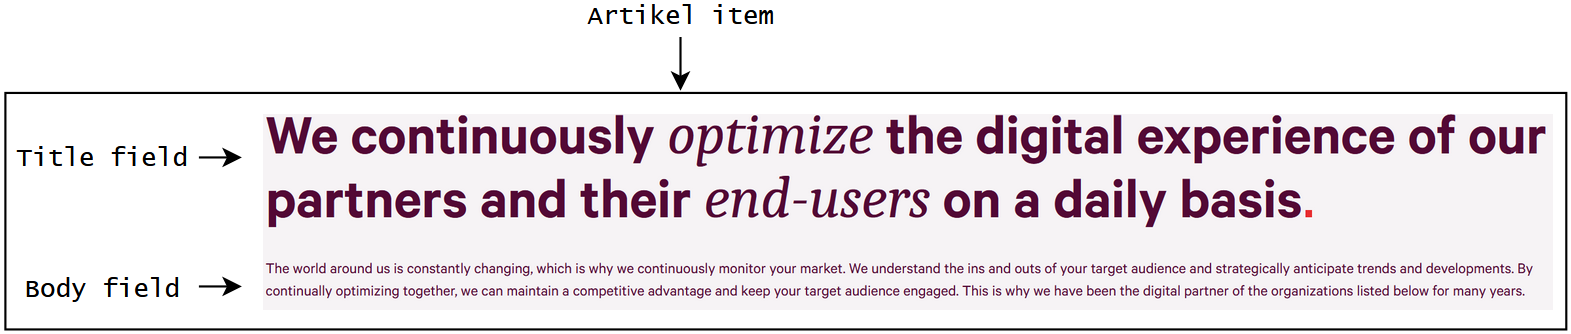
\includegraphics[scale=0.35]{VisualisationItems.png}
    \label{fig:VisualisationItems}
\end{graphic}

\whitespace
In het voorbeeld (figuur \ref{fig:VisualisationItems}) is te zien dat het item \qw{Artikel} 2 fields heeft.
Deze fields zijn \qw{Title} en \qw{Body} en bevatten de teksten voor de gedefinieerde gedeeltes van het item.
Een ander functionaliteit van een item is dat het meerdere items kan bevatten. 
Door dit te doen is het mogelijk om complexe structuren op te bouwen.
Voor deze structuur is ook een klassen diagram gemaakt wat te zien is in figuur \ref{fig:ClassDiagramItemField}.
Het datatype \qw{Content} zou verschillende primaire types kunnen bevatten zoals integer, string, boolean ect..
Dit kan per programmeertaal anders opgelost worden daarom is ervoor gekozen om de implementatie mogelijkheden niet te noteren.

\whitespace[2]
\begin{graphic}
    \captionsetup{type=figure}
    \caption{Visualisatie van een item}
    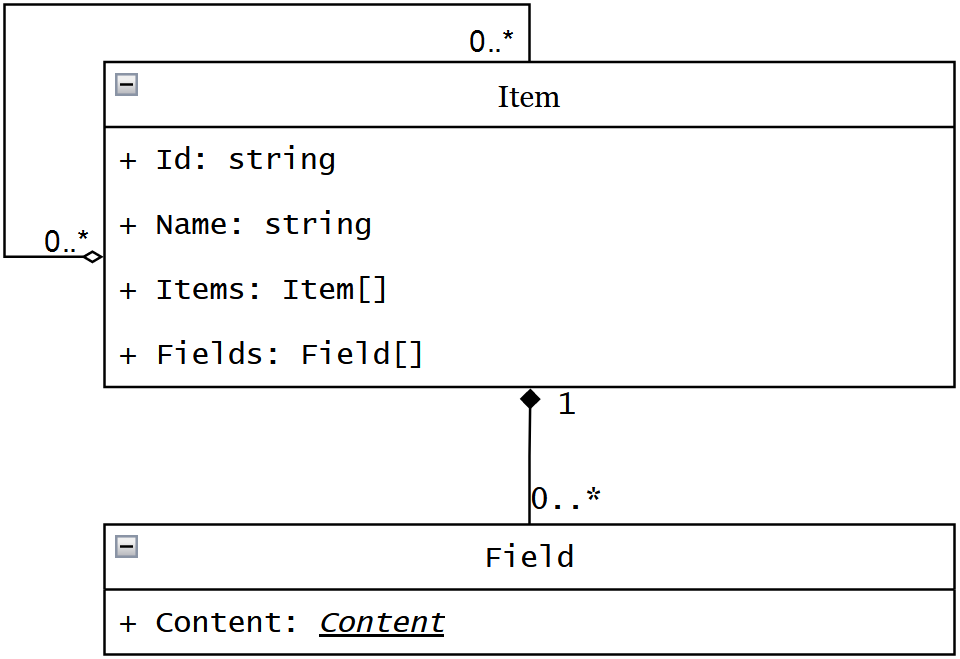
\includegraphics[scale=0.35]{ClassDiagramItemField.png}
    \label{fig:ClassDiagramItemField}
\end{graphic}
%
% \whitespace
% \textbf{Ontwerp Notes?}
%
% \whitespace
% Er is overwogen om meer richting een composite pattern te implementeren.
% Het ontwerp bestaat uit verschillende onderdelen met verschillende taken.
% Er wordt op elk onderdeel ingezoomd om een beter beeld te schetsen aan het ontwerp.
%
% \whitespace[2]
% \textbf{De content}
%
% \whitespace
% Om de content op te slaan wordt er gebruikgemaakt van een geneste structuur.
% Om deze geneste structuur op te bouwen is er gekozen om de data op te delen in 2 groepen.
%
% \whitespace
% \begin{itemize}
%     \item[1] \textbf{Simpele data}: hier worden de basis types van het systeem in opgeslagen.
%     Dit zijn de primaire types van de content voorbeelden van deze types zijn tekst, nummer en boolean.
%     In het ontwerp is simpele data genoteerd als \textbf{fieldvalues}.
%     \item[2] \textbf{Complexe data} is een samenstelling van 0 of meerdere \textbf{fieldvalues}.
%     Verder kan complexe data meerdere complexe data bevatten. 
%     Hierdoor kunnen er complexe structuren gemaakt worden.
%     Dit is gerepresenteerd als \textbf{ItemValues} in het ontwerp.
% \end{itemize}
%
% \whitespace
% Om structuur aan de data te geven worden ze voorzien door een definitie.
% Er zijn definities voor \textbf{itemvalues} en \textbf{fieldvalues}.
% Dit is gedaan zodat als er een nieuwe instantie van een stuk complexe data gemaakt moet worden dat dit op basis van de definitie gedaan kan worden.
% Om dit weer te geven is er een klassendiagram gemaakt die te zien is in figuur \ref{fig:DeContentClassDiagram}.
%
% \whitespace[2]
% \begin{graphic}
%     \captionsetup{type=figure}
%     \caption{Klassendiagram ItemValue}
%     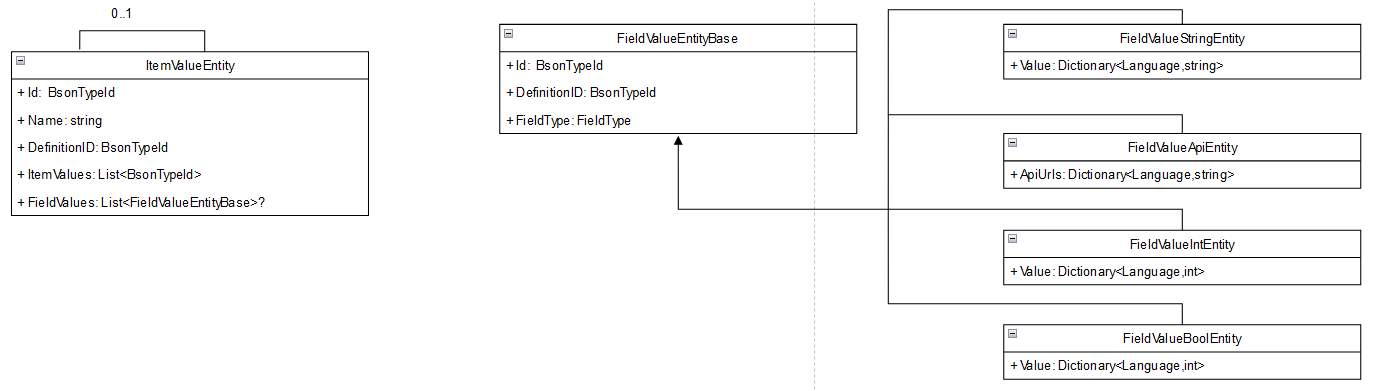
\includegraphics[scale=0.35]{ItemValueEntityClassDiagram.png}
%     \label{fig:DeContentClassDiagram}
% \end{graphic}
%
% \newpage
%
% \whitespace
% \textbf{De componenten}
%
% \whitespace
% Om de content een vorm te geven wordt er gebruik gemaakt van componenten.
% Voorbeelden van componenten zijn card, artikel en afbeelding.
% Door de componenten en de content te scheiden van elkaar geeft dat de mogelijkheid om verschillende componenten te gebruiken op hetzelfde stuk content.
% Om ervoor te zorgen dat een component een stuk content kan interperteren wordt er gebruik gemaakt van definities.
% Als een stuk content alle \textit{required FiedlDefinitions} heeft kan de component de content renderen.
% De componenten worden gerepresenteerd door \textbf{visualcomponent} in het ontwerp. 
% Een klasse diagram van de visual component is te zien in figuur \ref{fig:VisualComponentEntityClassDiagram}.
%
% \whitespace[2]
% \begin{graphic}
%     \captionsetup{type=figure}
%     \caption{Klassendiagram VisualComponent}
%     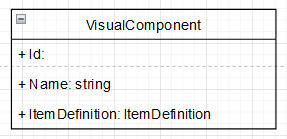
\includegraphics[scale=0.8]{VisualComponentEntityClassDiagram.png}
%     \label{fig:VisualComponentEntityClassDiagram}
% \end{graphic}
%
% \whitespace
% \textbf{De visualalisatie}
%
% \whitespace
% Om content op een pagina te renderen moet de content gekoppeld worden samen met de componenten.
% Dit wordt gerepresenteerd door het \textbf{itemvisual} in het ontwerp.
% Verder kan een itemvisual ook meerdere itemvisuals bevatten waardoor er een geneste structuur ontstaat.
% Hierdoor is het mogelijk om complexe websitestructuren te maken.
% Verder wordt ook op het itemvisual stijling en layout meegegeven zodat dit niet component afhankelijk is.
% Het klassen diagram voor het gehele ontwerp is te zien in figuur \ref{fig:ClassDiagramEntireSystem}
%
% \newpage
% \begin{graphic}
%     \captionsetup{type=figure}
%     \caption{Klassendiagram ItemValue}
%     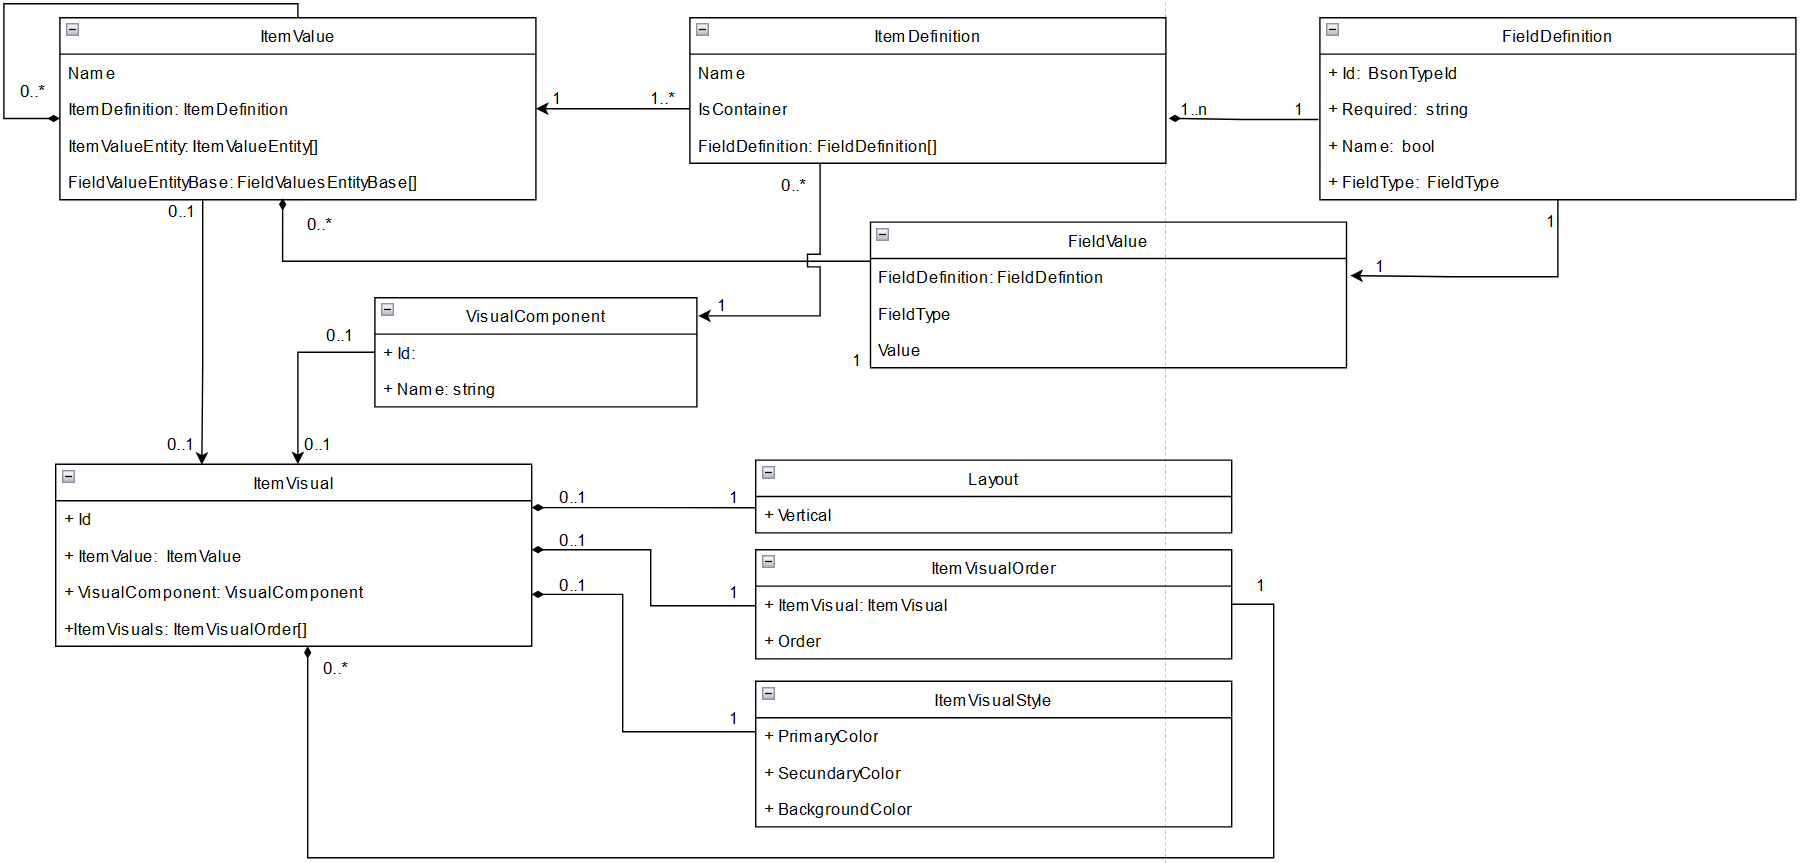
\includegraphics[scale=0.45,angle=90]{ClassDiagramEntireSystem.png}
%     \label{fig:ClassDiagramEntireSystem}
% \end{graphic}
